\section{Tests}
Les tests sont incontournables, ils permettent de verifier que les fonctions respectent leur signature.

\subsection{Utilisation de Jest}
L'un des objectifs de ce projet était de découvrir et prendre en main le framework Jest. Ce dernier est un environnement de travail pour réaliser des tests sous JavaScript (et compatible avec TypeScript). On a de nombreuses fonctions à disposition pour faire les tests notamment \texttt{test}, \texttt{expect} et \texttt{toBe}. Jest offre un affiche clair des tests qui passent ou pas, ce qui permet une correction rapide.

\subsection{Les fonctions et leur tests}
Les personnes faisaient les tests des fonctions qu'ils programmaient dans un soucis de performances. En effet une personne qui implémente un fonction connaît déjà les entrées et sorties de celle-ci donc peut faire les tests plus rapidement. Cependant nous avons remarqué que des cas limites sont oubliés ou pire encore que les tests sont faux car implémentés d'une façon trop proche à celle de la fonction.

Prenons l'exemple illustré par la figure~\ref{fig:ex_autre_tests}. Celui qui a codé la fonction \texttt{flip\_tile} (qui permet de tourner la tuile) a permuté les routes sans les tourner c'est-à-dire juste comme les quartiers. Les tests réalisés vérifiaient juste que les routes étaient permutées mais pas qu'elles étaient encore correctement connectées les une au autre. Donc les tests validaient une fonction incorrecte. Ainsi il vaut mieux qu'une autre personne fasse les tests même si c'est plus long.

\begin{figure}[H]
    \centering
    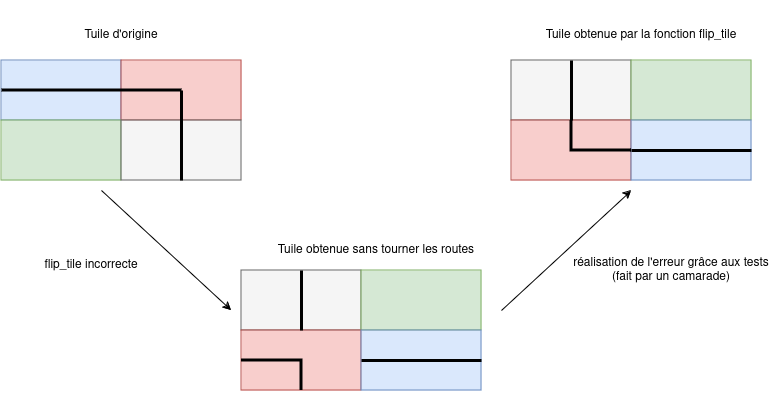
\includegraphics[width=0.8\linewidth]{images/tests/autre_fait_test.png}
    \caption{Problème du test fait par la personnes qui a codé la fonction}
    \label{fig:ex_autre_tests}
\end{figure}

Pour tester certaines fonctions, notamment celle dans \texttt{src/objectives.ts}, nous avions besoin d'avoir une partie reproductible, dont le résultat est attendu. Pour cela, nous avons utilisé le concept de \texttt{seed}~: pour une \texttt{seed} donnée, la partie jouée est la même. C'est l'identifiant d'une partie.

\subsection{Couverture}

La couverture du code est une métrique qui peut vous permettre de comprendre la part testée de nos sources, elle permet une meilleur fiabilité de celles-ci, en effet un code testé à 80\% donnera plus confiance en son utilisation qu'un code pas testé du tout. Afin de savoir le pourcentage de fonctions que nous testons il nous faut utiliser l'option \texttt{--coverage} sur la commande \texttt{npx jest}, la figure~\ref{fig:couverture} montre la couverture de nos tests.
Cette figure nous montre uniquement ce que nous testons mais pas si nos tests sont pertinents. Cependant comme nous pouvons le voir nos sources sont testés à 92\% ce qui assure au moins une certaine stabilité et fiabilité du code.

\begin{figure}[H]
    \centering
    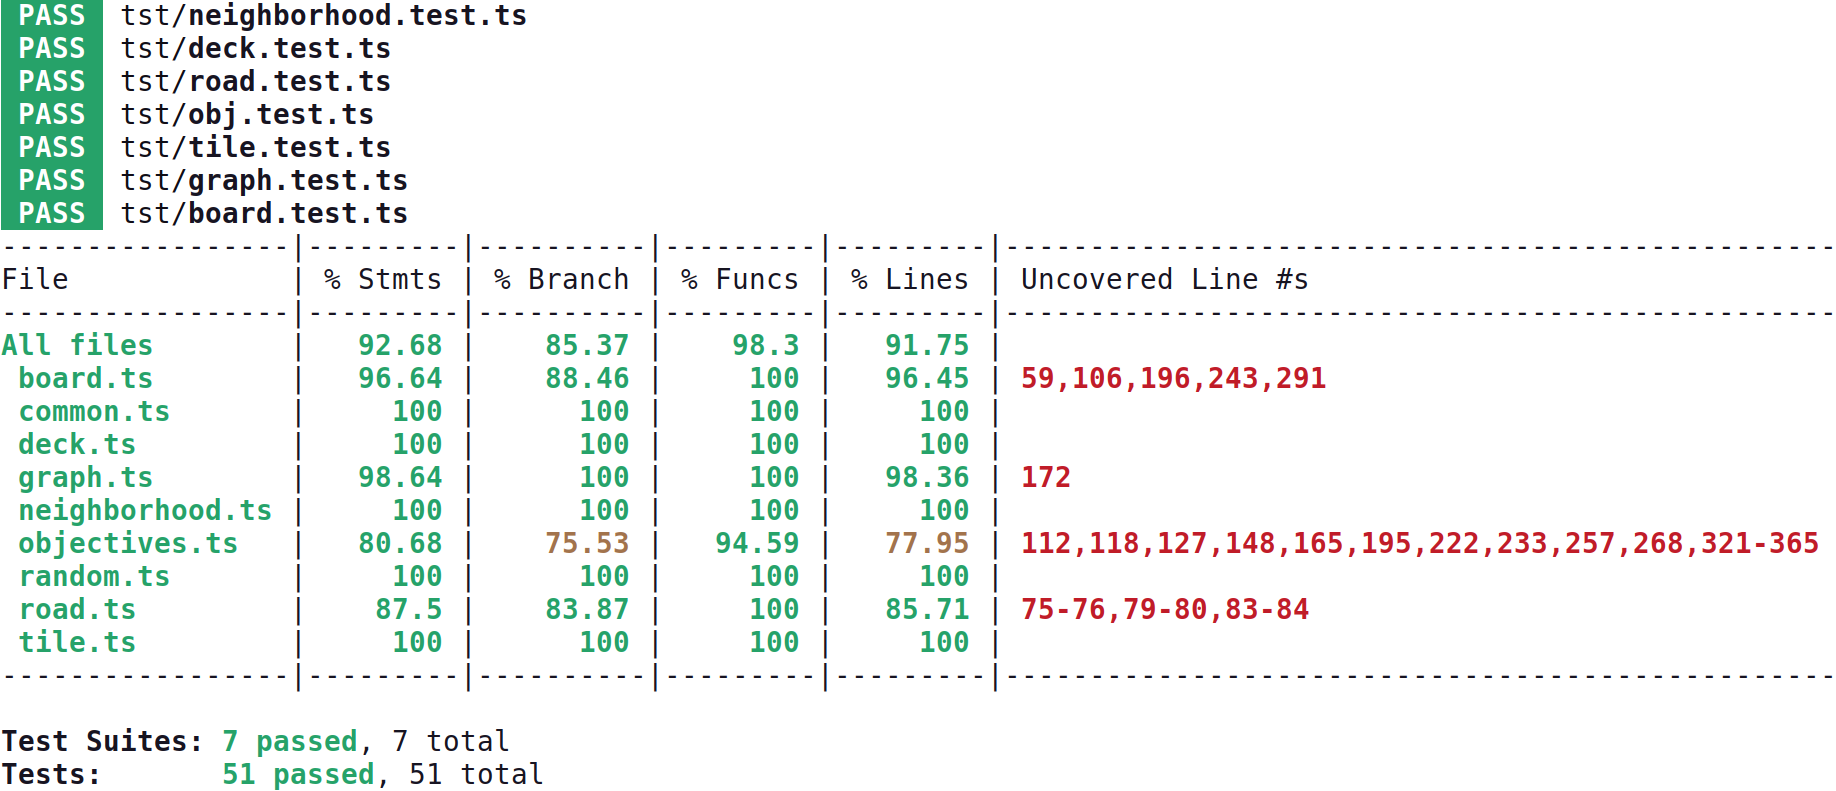
\includegraphics[width=0.9\linewidth]{images/tests/couverture_test.png}
    \caption{Couverture de nos tests}
    \label{fig:couverture}
\end{figure}